% Figure from MATH 591 notes, section 52. Compile with the notes preamble.
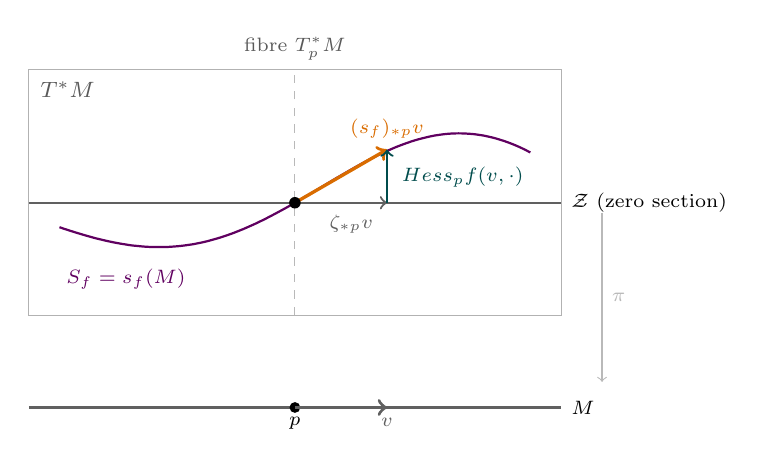
\begin{tikzpicture}[scale=1.3]
\draw[gray!60] (0,0.9) rectangle (5.2,3.3);
\node[font=\footnotesize, gray!70!black, anchor=north west] at (0.02,3.28) {$T^*M$};
\draw[thick, gray!75!black] (0,2.0) -- (5.2,2.0) node[right, font=\scriptsize, text=black] {$\mathcal{Z}$ (zero section)};
\draw[gray!55, dashed] (2.6,0.9) -- (2.6,3.3) node[above, font=\scriptsize, text=gray!70!black] {fibre $T_p^*M$};
\draw[violet!75!black, thick] plot[smooth] coordinates {(0.300,1.761) (0.350,1.744) (0.400,1.728) (0.450,1.712) (0.500,1.697) (0.550,1.682) (0.600,1.668) (0.650,1.654) (0.700,1.642) (0.750,1.630) (0.800,1.619) (0.850,1.609) (0.900,1.600) (0.950,1.592) (1.000,1.584) (1.050,1.579) (1.100,1.574) (1.150,1.570) (1.200,1.568) (1.250,1.567) (1.300,1.567) (1.350,1.568) (1.400,1.571) (1.450,1.575) (1.500,1.580) (1.550,1.587) (1.600,1.594) (1.650,1.604) (1.700,1.614) (1.750,1.626) (1.800,1.640) (1.850,1.654) (1.900,1.670) (1.950,1.687) (2.000,1.705) (2.050,1.725) (2.100,1.745) (2.150,1.767) (2.200,1.789) (2.250,1.813) (2.300,1.837) (2.350,1.863) (2.400,1.889) (2.450,1.916) (2.500,1.943) (2.550,1.971) (2.600,2.000) (2.650,2.029) (2.700,2.059) (2.750,2.088) (2.800,2.118) (2.850,2.148) (2.900,2.178) (2.950,2.208) (3.000,2.238) (3.050,2.267) (3.100,2.296) (3.150,2.325) (3.200,2.353) (3.250,2.381) (3.300,2.408) (3.350,2.434) (3.400,2.459) (3.450,2.483) (3.500,2.506) (3.550,2.528) (3.600,2.549) (3.650,2.568) (3.700,2.586) (3.750,2.603) (3.800,2.618) (3.850,2.631) (3.900,2.643) (3.950,2.654) (4.000,2.662) (4.050,2.669) (4.100,2.674) (4.150,2.677) (4.200,2.678) (4.250,2.677) (4.300,2.674) (4.350,2.670) (4.400,2.663) (4.450,2.655) (4.500,2.644) (4.550,2.632) (4.600,2.617) (4.650,2.601) (4.700,2.583) (4.750,2.563) (4.800,2.541) (4.850,2.517) (4.900,2.491)};
\node[violet!75!black, font=\scriptsize] at (0.95,1.25) {$S_f = s_f(M)$};
\draw[->, very thick, orange!85!black] (2.6,2.0) -- (3.5,2.520) node[above, font=\scriptsize] {$(s_f)_{*p}v$};
\draw[->, thick, gray!75!black] (2.6,2.0) -- (3.5,2.0);
\draw[->, thick, teal!60!black] (3.5,2.0) -- (3.5,2.520);
\node[teal!60!black, font=\scriptsize, anchor=west] at (3.55,2.250) {$\operatorname{Hess}_p f(v,\cdot)$};
\node[gray!75!black, font=\scriptsize, anchor=north] at (3.1500000000000004,1.98) {$\zeta_{*p}v$};
\fill (2.6,2.0) circle (1.6pt);
\draw[thick, gray!75!black] (0,0) -- (5.2,0) node[right, font=\scriptsize, text=black] {$M$};
\fill (2.6,0) circle (1.5pt) node[below, font=\scriptsize] {$p$};
\draw[->, very thick, gray!75!black] (2.6,0) -- (3.5,0) node[below, font=\scriptsize] {$v$};
\draw[->, gray!55] (5.6,1.9) -- node[right, font=\scriptsize] {$\pi$} (5.6,0.25);
\end{tikzpicture}
